%voor Kim: http://thesaurus.com/browse/therefore

\section{Theoretical background}
\subsection{Features}
A 'feature' represents a characteristic of a voxel and its environment. Lists of
features for all the voxels in an image are used to describe the entire image.

\subsubsection{Feature extraction}
Feature extraction involves obtaining a list of feature from a resource -- an
image or another dataset -- to describe that dataset in an accurate way which
allows it to be analysed by proper software.

In image processing a wide range of features can be extracted. Some features are
very trivial: the grey value or colour of pixels, the position of pixel, etc.
Features also can be shape based: template matching, blob detection, edge
detection, detection of lines and circles by means of a Hough transform, etc.
Once certain objects are detected in the image, their area, curvature, size,
etc. can be determined.

%TODO does this belong under extraction?
We will now highlight some of the most relevant features for our purpose.

\paragraph{Distance Map}
A binary image containing either foreground (1) or background (0) voxels can be
transformed into a distance map. In this process, every foreground voxel is
assigned the distance to nearest background voxel, while the background voxels
are simply set to zero. In that regard, distance maps can be seen as
generalisations of edges: they contain the same information, and more. An
exanple of a distance map can be found in \autoref{fig:distmap}.

\begin{figure}[htp]
\begin{center}
  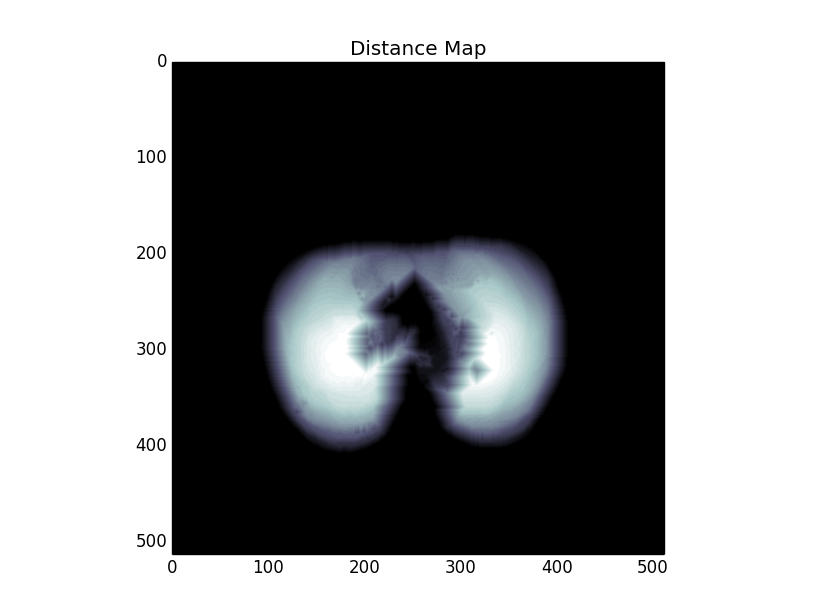
\includegraphics[width=\linewidth]{img/distmap.png}
  \caption{Example of a distance map}
  \label{fig:distmap}
\end{center}
\end{figure}

The distance metric must not necessarily be the Euclidean distance. Other
metrics such as the Manhattan distance are also acceptable and easier to compute
on top of that.

\paragraph{Laplacian}\label{sec:laplace_theory}
One common feature in nodule detection is the laplacian -- also called blob
detector. The laplacian operator applied to a continuous 3D function is
defined as:

\begin{equation}
	\nabla^2f(x,y,z) = \left(\frac{\partial^2 f}{\partial x^2} + \frac{\partial^2
	f}{\partial y^2} + \frac{\partial^2 f}{\partial z^2}\right)
\end{equation}

To be applied to images, it must first be discretized into a 3D convolution
mask. That mask typically has a large negative number in the center, surrounded
by positive ones.

Because we are dealing with second derivatives, this operation is very sensitive
to noise. One solution to this problem is to convolve the image with a gaussian
kernel of scale $t$ first. Because this kernel has a low-pass effect, noise will
be reduced.

\begin{equation}
	G_t(x,y,z) = \frac{1}{(\sqrt{2\pi} t)^3}e^{-\frac{x^2+y^2+z^2}{2t^2}}
\end{equation}

It can be represented by bionomial filters -- repeated convolutions of [1 1]
with itself -- in the discrete domain, making it rather cheap operation
computation-wise.

Convolution has some interesting properties, which allow this calculation to be
further optimized:

\begin{equation}
	\nabla^2[G_t(x,y,z) * f(x,y,z)] = \nabla^2 G_t(x,y,z) * f(x,y,z)
\end{equation}

The $\nabla^2 G_t(x,y,z)$ term is often referred to as the Laplacian-of-Gaussian
(LoG) or Mexican hat filter. The LoG can be used to detect edges by finding its
zero crossings, but we are more interested in its blob detection capabilities.
It results in a strong positive response for dark blobs of uniform intensity
with extent $\sqrt{2t}$ on a light background and vice versa for light blobs on
dark background. The latter description fits most, if not all, nodules.

To get this strong response, we must carefully calibrate the scale parameter $t$
to the nodule radius. However, because nodules come in different sizes, $t$ will
likewise have to range over different values. In general, larger $t$ values
yield lower filter responses. This makes finding minima and maxima in
scale-space difficult. Using the scale-normalised laplacian operator solves this
problem by multiplying the response with $t$.

To make this computationally expensive operation more bearable, the laplacian is
often approximated by the difference between two levels in a gaussian scale
pyramid. The result is called the Difference-of-Gaussians (DoG).

There is one last technicality we must address. The above formulas assumed
that the blobs were isotropic and thus that the LoG could be so as well.
However, because we perform most of our calculations in voxel space and voxels
are not perfect cubes, this assumption does not hold. To compensate for this
fact, we define a unique sigma per dimension that is a rescaled variant of the
original based on the corresponding voxel dimension.

Alternatively to the laplacian, one can also use the Hessian matrix of second
partial derivatives as a feature. The laplacian is simply the sum of the
elements on the Hessian's main diagonal. In that sense the latter is more
complete, but also much more computationally expensive. For this reason, we
stick with the laplacian operator.

\paragraph{3D Averaging}\label{sec:3davg} 
This method \cite{keshani} is based on the fact that nodules are
more or less spherical while bronchi and bronchioles are oblong. This might not be
visible in a 2D image where both appear as spheres depending on the
orientation of the bronchioles, but it certainly is if a 3D volume around a
finding is taken into account. Larger nodules will repeat themselves in the
preceding and/or succeeding slices at the same place while the smaller bronchi
and bronchioles will not. For small nodules hidden in a maze of brionchioles of
the same diameter, the separation is done based on the fact that the small
nodules will not continue in preceding and/or succeeding slices while the
bronchioles will. Thus, by comparing the grey value of the target voxel with the
grey values found in the neighbour slices at the same place and by taking into
account the difference in length between nodules and bronchioles the nodules can
be separated from the other findings. The comparison was made by calculating the
mean value of each window in the target slice, the average of the mean values of
the same coordinates in the succeeding and preceding slices:
\begin{equation}
M_{ij}^p = \frac{1}{9} \sum_{k,l = -1}^{+1} L^p(i+k,j+l)
\end{equation}
\begin{equation}
M_{ij}^{+} = \frac{1}{q} \sum_{p=p+1}^{p+q} M^p_{ij}
\end{equation}
\begin{equation}
M_{ij}^{-} = \frac{1}{q} \sum_{p=p-q}^{p-1} M^p_{ij}
\end{equation}
\begin{equation}
\text{3D averaging} = M^{-}_{ij} M^{+}_{ij} 
\end{equation}

The index $p$ indicates the z-index of the slice and the parameter $q$ is the number
of slices that are considered. The latter parameter is calculated as the ratio
of the estimated nodule length to the thickness of the slices.
\begin{equation}
q=\frac{c}{T}
\end{equation}
To differentiate between larger nodules and small bronchioles and between
smaller nodules and similar bronchioles the parameter $c$ was set at 5mm and 2,5mm
respectively. The window around each voxel was set at $3 \times 3$. In case of a high $q$ a
high 3D averaging score will classify a voxel as belonging to a nodule whereas a
low score will classify a voxel as a non-nodule. For the low $q$ value it is the
opposite.

\subsubsection{Feature selection}
A problem that may arise when analysing a dataset based on list of features, is
that the amount of features is too large. Performing an analysis on large amounts
of datasets requires a large amount of memory and computational power.
Furthermore, a classification algorithm that is used to analyse the data may
overfit the training data and will not be able to generalise anymore.
Therefore, a range of dimension reduction techniques can be applied to extract
the uncorrelated and most important features of a list. Examples of these
reduction techniques are principal component analysis and partial least squares
regression. %TODO relevant?

\subsubsection{Features in nodule detection} \label{sec:featureselection}
A non-exhaustive literature review revealed some commonly used features used in
automatic nodule detection. \cite{tartar} primarily used morphological features:
area, perimeter, diameter, solidity, eccentricity, aspect ratio, compactness,
roundness, circularity and ellipticity. To select these features the minimum
Redundancy Maximum Relevance (mRMR) method was applied. Selecting relevant
features is import to improve the accuracy of the algorithm and to reduce the
processing time. \cite{mur} used 3D local image features which were calculated
per voxel: shape index and curvedness. \cite{chen} calculated the size, margins,
contours and internal characteristics of the candidate nodules. \cite{keshani}
used 2D stochastic features �grey level values and intensity values-  as well as
3D anatomical features to remove the bronchioles from the list of candidate
nodules. The features selected by \cite{teramoto} were area, surface area,
volume, CT value, convergence, diameter and overlapping area. The algorithm of
\cite{ozekes} implemented 3D features such as straightness, thickness, vertical
and horizontal widths, regularity and vertical and horizontal black pixel
ratios.

These features are calculated based on a prior segmentation of the nodules. On
the other hand, instead of doing a nodule segmentation first, a lot of features
can be calculated on the image itself based on grey values, intensities,
grey values in the neighbourhood, etc. Although this is not a very common
approach, these features can be generated without any preprocessing of the
image and can then be fed to a classifier to calculate a nodule-probability for
each voxel.


\subsection{Machine learning}
The research field of machine learning is dedicated to the automatic
learning of software in order to make accurate predictions based on past
observations \cite{mach}. This concept is of course very interesting when
detecting nodules as a vast amount of 'past observations' are available.
Classifiers are algorithms that classify given examples into a given set of
categories \cite{mach}. CAD systems which implement a classifier tend to
outperform the CAD systems which do not \cite{lee2010}. Therefore, the use of
classifiers is very common in this field of research and many classifiers have
been tested.

\subsubsection{Classifiers used in nodule detection systems}
\cite{caruana} compared the performance of a range of classifiers on eleven
binary classification problems. The supervised learning algorithms that were
used are SVM, NN, Naive Bayes, Memory-Based Learning, RF, Decision Trees, Bagged
Trees, Boosted Trees and Boosted Stumps. Prior to calibration Bagged Trees, RF
and NN perform the best on average across all test problems. After calibration
Boosted Trees outperformed all other methods. The performances of SVM, Boosted
Stumps and Naive Bayes were also dramatically improved by calibration. The
performance of RF was not increased significantly. Overall, \cite{caruana}
suggests calibrated boosted trees is the best learning algorithm. RF are close
second, followed by uncalibrated bagged trees, calibrated SVM and uncalibrated
NN. However, the training of Boosted Trees is inherently sequential which makes
it slower to implement than RF. Another problem may be the noisyness of the
data. Therefore, the choice and tuning of the parameters of the boosted trees
(depth of trees, amount of trees, etc.) algorithm should be done carefully and
this will take some time.

SVM are widely used in the development of nodule detection CAD systems
\cite{keshani, lee2010, ozekes}. According to \cite{ash} SVM even outperforms
RF. However, SVM has some disadvantages. First of all, the featues to be used
need to be determined in advance and there is no such thing as a standard
feature set (see also \autoref{sec:featureselection} ). In the ideal case these
features should all have the same dimensions and/or magnitudes. With SVM
problems may arise with noisy data and images are very often quite noisy. The
time complexity of SVM is $O(n^2)$ \cite{svmcompex}.

The best performing CAD system in the ANODE09 challenge, which is entirely
dedicated to comparing nodule detection CAD systems, was the ISI-CAD algorithm
\cite{ginneken}. ISI-CAD uses a k-nearest neighbour classifier to reduce the
amount of FPs which has the disadvantage that the features should all be of the
same magnitude in order to perform an optimal classification.

 
\subsubsection{Random Forests, an ensemble classifier }
Ensemble learners combine decisions of multiple classifiers to form an
integrated output \cite{lee2010}. The use of multiple learning algorithms at the
same time has the advantage that a better predictive performance is obtained
compared to the predictive performance demonstrated by each individual learning
algorithm separately.

Random Forests (RF) is a relatively new classification method which has not been
exhaustively explored yet. ``Random Forests are a combination of tree predictors
such that each tree depends on the values of a random vector sampled
independently and with the same distribution for all trees in the forest. The
generalisation error for forests converges to a limit as the number of trees in
the forest becomes large.'' \cite[~p.5]{breiman} For this reason RF is an ensemble
learning method. So given a test sample as the input, this input vector is put
down each of the trees, each tree gives a classification and the forest selects
the classification that has most votes. Consequently, the output of the RF
depends on the combination of results from all individual trees. In this way a
variance reduction is achieved and the output is made more robust against noise
\cite{breiman, lee2010, RFcompex}. RF has the advantage that the set of features
do not need to be known in advance as the algorithm itself decides on itself
which features to use. Therefore, a lot of features can be generated at will and
the algorithm itself will decide on using them or not. The time complexity of RF
is $O(n \log n)$ \cite{RFcompex} which makes it more suitable than e.g. SVM for
large datasets.

However, although the RF classifier might be a good choice for analysing large
datasets because of the fact that a large amount of features can be used and
because of the rather limited time complexity compared to other classifiers, the
amount of memory and computational power can still be a problem. Hence, an
optimisation of the implementation of the RF classifier can be desirable. A
possible optimisation is the use of a cascaded classifier.

\subsubsection{Cascaded classifiers}
A cascaded classifier exists of several classifiers at different levels that are
concatenated. Consequently, it is a special case of an ensemble classifier. The cascaded
classifier uses all the information that is obtained in a previous level to
provide the classifier in the next level with additional info on the data. On a
lower level in a cascaded classifier the amount of features and the complexity
of the features that are used are lower.
For example, the first feature in a classifier used to classify the voxels of a
3D image into two classes -- nodules or non-nodules -- is the grey value of each
voxel. This is a feature we get for free as it is readily available without
performing any calculations. The classifier at the first level determines a
threshold to separate nodule voxels from non-nodule voxels based on their grey
values. Using this trivial feature a large part of the voxels can already be
eliminated as their grey value is too high or too low to be a nodule voxel. The
features on the second level are more complex and therefore require more
computational power. However, this is not a problem anymore as the amount of
voxels to be processed was reduced after the first level. At the second level
again a number of voxels are eliminated. The number of levels, and therefore the
number of features, can be increased until the end results are satisfying: all
voxels are classified (correctly) into x amount of classes. However, classifying
all voxels in the correct class is not trivial and some voxels might be
classified in the wrong class. Which amount of false positives and false
negatives is acceptable is to be decided by the user.

The reason for using a cascaded classifier is that both memory and CPU time are
often limited. By discarding a certain amount of non-nodules at each level of
the classifier, it is not necessary to calculate all features for all nodules
which saves memory and CPU time.

The performance of the classifier depends on the features that are implemented
on each level. For data mining the general rule is the more the better. If a lot
a features are provided for each voxel the classifier can set more thresholds
and is therefore better able to separate different classes. We started off from
this concept, but very soon we had to deal with memory errors in Python. The
code was therefore optimised, but still we had to cut in the amount of features
that were used in the final version of the classifier as the amount of memory
available remained a problem during the whole project.

\subsection{Validation metrics}
In order to evaluate the performance of a binary classifier, we introduce some
statistical concepts. The reader should be familiar with Type I and Type II
errors. A Type I error occurs when the model predicts something to be there
while in reality it is not. In this text we call these occurences false
positives (FP). In our scenario, this corresponds with a classifier indicating
that a nodule is present when there is really none.

Vice versa, a Type II error occurs when the model predicts something to be absent
when in reality it present. We call them false negatives (FN). False negatives
in our scenario represent nodules not detected by the classifier.

Of course the classifier does not always have to be wrong. True positives (TP)
and true negatives (TN) respresent the cases where the classifier properly
detected the presence or absence of the nodule respectively.


\autoref{tbl:stats} summarizes these definitions.
\begin{table}[htp]
\begin{center}
	\begin{tabular}{r | c c}
						& Nodule 	& Non-Nodule \\
		    \hline
		    Positive 	& TP 		& FP\\
		    Negative 	& FN 		& TN \\
	\end{tabular}
	\caption{Summary of some basic statistical measures.}
	\label{tbl:stats}
\end{center}
\end{table}

Because the terms above are in absolute numbers, they are difficult to compare
across studies. That is where sensitivity and specifictiy come in. Sensitivity
compares the amount of true positives with the total amount of positives.
Synonyms include the true positive rate or the recall rate. Specificity does the
same for the negatives. It is sometimes also called true negative rate.

\begin{equation}
	\text{sensitivity} = \frac{TP}{TP + FP}
\end{equation}

\begin{equation}
	\text{specificity} = \frac{TN}{TN + FN}
\end{equation}

Ideally both measures should be 100\% but that is an unrealistic expectation.
There is also an inherent trade-off between the two: when the sensitivity is
increased to make sure no false positives are detected, this will also increase
the false negatives, which in turn lowers specificity. In our case there is a
clear preference for a higher sensitivity, even though it may cost us some
specificity.

One last important measure is the accuracy. It is the ratio of all correctly
classified occurrences over all occurrences.

\begin{equation}
	\text{accuracy} = \frac{TP + TN}{TP + FP + TN + FN}
\end{equation}

Ideally TP, FP, TN and FN should all be measured in the same units: either
voxels or nodules. Pure voxel classification schemes can simply calculate how
many voxels were correctly identified, while classification schemes working with
nodules can use the number of nodules. However, our approach is a hybrid of the
two. We don't require all voxels of the nodule to be detected to label the
nodule as TP, one (or a couple) should be plenty. Hence, our TP and FN are
expressed in number of nodules. This leaves us with a problem for FP and TN, as
these cannot be expressed in an amount of nodules. We somewhat alleviate this
problem by grouping clusters of voxels together, but the impact on our
measurements is still significant.